\section{Monte Carlo Simulations}
\label{sec:MonteCarloSims}

% TODO: Write about Monte Carlo sims

\section{Ergodicity}
\label{sec:Ergodicity}

An ergodic system is one where its time average coincides with its ensemble average. 

Intuitively, ergodicity is the assumption that a Markov chain starting from some state $S_a$ with a non zero Boltzmann weight can reach any other state $S_b$ withing a finite number of updates~\cite{Zwanzig:nonequil_stat_mech}.

This is necessary to assume, since otherwise there could be a non zero contribution to the partition function not being sampled by the Markov chain.

\section{Detailed Balance}
\label{sec:DetailedBalance}

Generally, a Markov process can be described through the Master equation

\begin{equation}
    \frac{\mathrm d P_a}{\mathrm d t} = \sum_{a \neq b} \left ( P_b W_{ba} - P_a W_{ab} \right )
\end{equation}

where $P_a$ is the probability to find the system in the state a, and $W_{ab}$ is the transition rate from the state $a$ to $b$. This equation describes the equilibrating of $P_a$ into $P_a^{eq} \propto e^{-\beta E_a}$. The resulting equation is called detailed balance

\begin{equation}
    W_{ba} e^{\beta E_b} = W_{ab} e^{\beta E_a}
\end{equation}

This describes an equal rate of flow into the state $a$ as out of it.

% TODO: Write dividing W_ab and write about acceptance ratio.

\section{Worm Algorithm}
\label{sec:WormAlgorithm}

% TODO: Write about worm algo from the article on Telegram



\section{Graph Dividing Algorithm}
\label{sec:GraphDivisonAlgorithm}

\begin{figure}[h!]
    \centering
        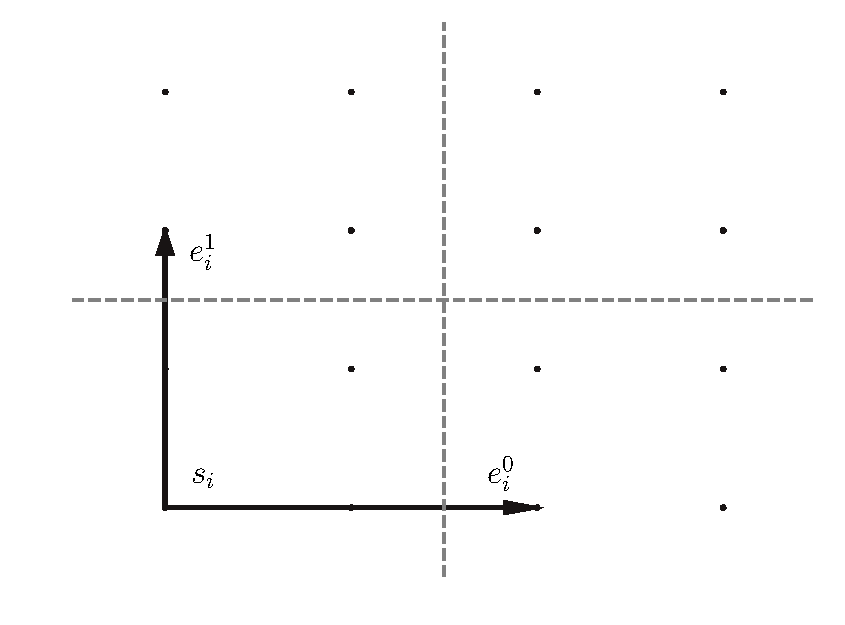
\includegraphics[width=0.8\textwidth]{figures/graphDividing.pdf}
    \caption{One step in the graph dividing algorithm where $l_i = 4$. $e^0_i$ and $e^1_i$ are drawn from site $s_i$. Summed permutations of $\{e^0_i, e^1_i\}$ give the starts for the next boxes. The next iteration of boxes are shown via the dividing dotted lines.}
    \label{fig:graphdividingalgo}
\end{figure}

In order to calculate the box dimension the lattice need to be divided into boxes of decreasing size. A step by step instruction of a graph dividing algorithm is provided below, and an implementation in pseudocode is available in the Appendix at Section \ref{sec:pseudocodeboxdivisionalgo}.

For brevity some abbreviations are introduced.

\begin{equation*}
    \begin{aligned}
        d =& \ \text{dimension} &\quad l_i =& \ \text{side length of the current box}\\
%
        l_0 =& \ \text{side length of the} &\quad e_i^j =& \ \text{vector of length } l_i / 2 \\
%
             & \ \text{smallest box allowed} & & \text{ in the }j\text{'th direction} \\
%
        \text{perm}(v) =& \ \text{All permutations of } v &\quad s_i =& \ \text{starting site of the current box}
    \end{aligned}
\end{equation*}

\begin{enumerate}
    \item If $l_i \geq l_0$, go to 2, else stop.
%
    \item Save all sites in the current box, starting for $s_i$ going $l_i$ in $d$ directions.
%
    \item Find all starting points for new boxes.
%
    \begin{enumerate}[label=(\roman*)]
%
        \item Form the matrix $E = (e_i^0, e_i^1, \  \ldots, e_i^d)^T$
%
        \item For all vectors $v_k$ in perm$(0, 0, \ \ldots , 0)$, perm$(1, 0, \ \ldots , 0)$, \\ \ldots, perm$(1, 1, \ \ldots , 1)$, create the new start $s_k$ as $$s_k = v_k E$$
%
    \end{enumerate}
%
    \item For each start $s_k$:
    \begin{enumerate}[label=(\roman*)]
        \item $s_i = s_k$, $l_i = l_i / 2$
        \item Go to 1.
    \end{enumerate}
%
\end{enumerate}

This algorithm can be written to perform in linear time, as can be seen in Figure (\ref{fig:bench_graphdiv}). 

\begin{figure}[h!]
    \centering
        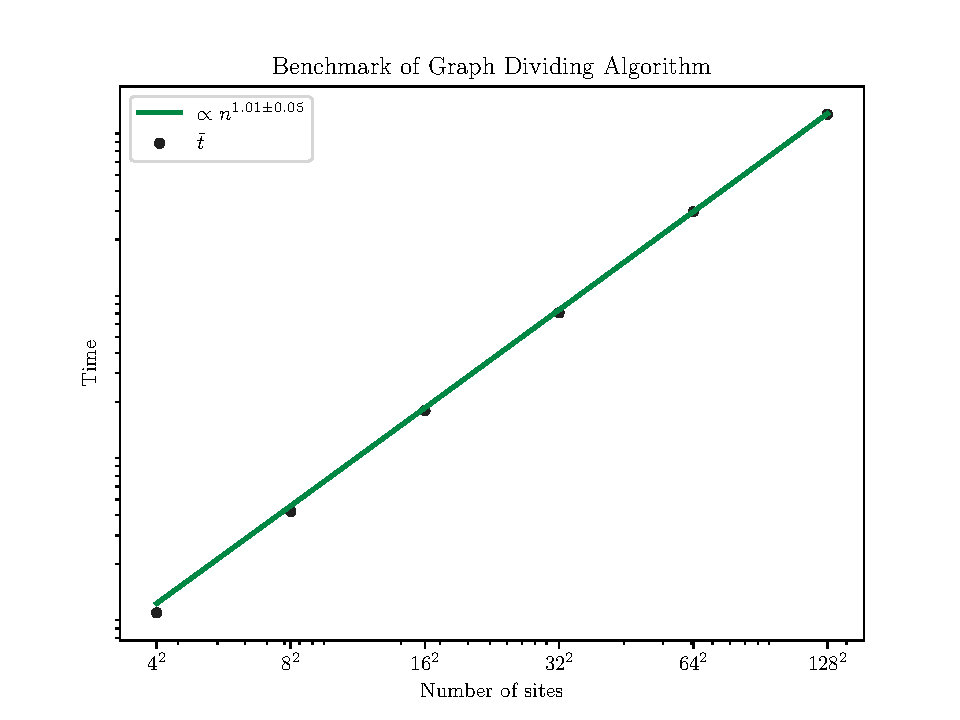
\includegraphics[width=0.8\textwidth]{figures/bench_graph_div.pdf}
    \caption{Loglog plot of a benchmark of the graph dividing algorithm. The y-axis show the time taken to perform one full graph divide normalized against the smallest time value.}
    \label{fig:bench_graphdiv}
\end{figure}

\section{Error Estimation}
\label{sec:ErrorEst}

In this thesis a number of error estimation techniques were used to know how much data was needed for each measurement. In this section the techniques will be described intuitively.

\subsection{Monte Carlo error estimation}
\label{subsec:MonteCarloErrorEst}

Given a Monte Carlo simulation where polling of some quantity $A$ has been done $N$ times an estimation of the expectation value of $A$ is

\begin{equation}
    \bar A = \frac{1}{N} \sum_{i = 1}^{N} A_i
\end{equation}

where each sampling was labeled $A_i$. To show that this is an unbiased estimator the expectation value of the difference between the estimation and the real value $\langle A \rangle$ is used.

\begin{align}
    \langle \bar A - \langle A \rangle \rangle &= \langle \bar A \rangle - \langle A \rangle \\
%
    &= \left \langle \frac{1}{N} \sum_{i = 1}^{N} A_i \right \rangle - \langle A \rangle \\
%
    &= \frac{1}{N} \sum_{i = 1}^{N} \langle A_i \rangle - \langle A \rangle \\
\label{eq:unbiasedEst}
%
    &= \frac{1}{N} \sum_{i = 1}^{N} \langle A \rangle - \langle A \rangle \\
%
    &= \frac{1}{N} N \langle A \rangle - \langle A \rangle = 0
\end{align}

where the fact that $A_i$ is a random sampling from the distribution of $A$ was used in (\ref{eq:unbiasedEst}).

The standard deviation of this estimate can be calculated through the variance.

\begin{align}
    \sigma_{\bar A}^{2} &= V\left( \bar A - \langle A \rangle \right ) \\
%
    &= V\left(\bar A\right) - V\left(\langle A \rangle\right) \\
%
    &= \{ \langle A \rangle \ \text{is a constant} \Rightarrow V(\langle A \rangle) = 0 \} \\
%
    &= V \left ( \frac{1}{N} \sum_{i = 1}^{N} A_i \right ) \\
%
    &= \{ \text{Monte Carlo simulations give independent samples} \} \\
%
    &= \frac{1}{N^2} \sum_{i = 1}^{N} V(A_i) \\
%
    &= \{ V(A_i) = \sigma_{A}^2 \} \\
%
    &= \frac{1}{N^2} N \sigma_{A}^2 = \frac{\sigma_{A}^2}{N}
\end{align}

or

\begin{equation}
    \sigma_{\bar A} = \frac{\sigma_A}{\sqrt{N}}
\end{equation}

So the standard error in this estimation decreases as $N^{-1/2}$.

\subsection{Bootstrap}
\label{subsec:Bootstrap}

Bootstrap is a resampling method to examine a probability distribution. In this thesis it was used to estimate the error propagation of parameters in curve fitting.

Given a set $\bm x$ of $N$ measurements from an unknown distribution $\hat \phi$, some statistical calculation of interest can be done as $\theta = s(\bm x)$. A resampling $\bm x_0$ of $\bm x$ comprised of $N$ random measurements from $\bm x$ (where one measurement can be included several times), can then be used to calculate $\theta^*_0 = s(\bm x_0)$. Repeating this $N_B$ times gives an estimate $\theta^* = (\theta^*_0, \theta^*_1, ..., \theta^*_{N_B})$ of the distribution $\hat \theta$. Assuming $N_B$ is large then, by the central limit theorem, $\hat \theta$ is a normal distribution with some standard deviation $\sigma_\theta$ that can be used as an error estimation for $\theta$.

\section{Optimization}
\label{sec:Optimization}

A large part of this project was spent optimizing the simulations. To fascilitate this process, the Google project \textit{benchmark} was used for measuring and comparing running times of different algorithms. Only the C++ code was optimized, since the prototypes written in Python were not concerned with computational speed. What follows is a summation of the biggest optimizations that were achieved during this project.

\subsection{Lattice implementation - Squashing the Graph}
\label{subsec:LatticeImpl}

During most of the calculations a sweep through the entire lattice was necessary. The computational time taken by such a sweep is heavily affected by the implementation of the lattice data structure.

The first implementation used an array of arrays to represent the lattice. This has the advantage of a similar interface to mathematical matrices with rows and columns. This is however much slower than a single array, or a squashed graph, most likely due to cache misses\cite{Hanlon:CacheMisses}. Figure (\ref{fig:bench_latticeimpl}) shows a comparison between the time it takes to do one full sweep in the two implementations.

Furthermore, this simplifies the generalization to lattices of different dimensions since the need to allocate a set number of arrays in each array disappears. It also makes it easier to reuse the same algorithm for lattices of different dimensions.

The mapping used between the array index and the Euclidean space is

\begin{equation}
    n = x + y L + z L^2 + ...
\end{equation}

where $L$ is the linear system size.

\begin{figure}[h!]
    \centering
        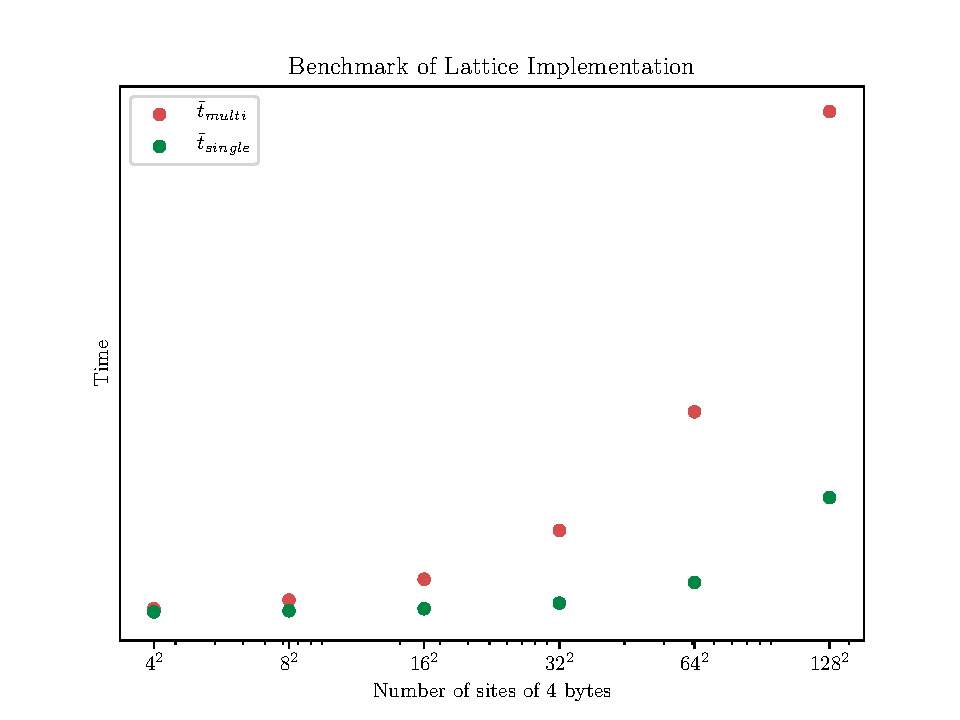
\includegraphics[width=0.8\textwidth]{figures/bench_latticeimpl.pdf}
    \caption{Plot of a sweep benchmark of two different lattice implementations. The red dots labeled $\bar t_{multi}$ is an array of arrays, while the green dots labeled $\bar t_{single}$ is a single array. The y-axis show the time taken to perform one full graph divide normalized against the maximum of the smallest time value for the two implementations.}
    \label{fig:bench_latticeimpl}
\end{figure}

\section{Testing}
\label{sec:Testing}

Testing is an essential part of writing a simulation. The correctness of the code ensures that the physical model is aptly described. To facilitate the development, a number of coding practices were applied, such as unit testing (Section \ref{sec:UnitTesting}) and regression testing (Section \ref{sec:RegressionTesting}). The tests for the prototypes were written in the Python standard library utility \textit{unittest}, and those for the main simulation used the C++ framework \textit{Catch2}.

\subsection{Unit Testing}
\label{sec:UnitTesting}

Unit testing refers to the practice of isolating a `unit' of code and testing its correctness. A unit can be any small piece of code with an expected behaviour.

This was done by manually calculating the expected output of some code, given some input, and ensuring that the piece of code produced an equivalent result.

The parts of the simulation using a pseudorandom number generator were tested by randomly selecting a set of seeds on which the tests were run upon. The correctness is then assumed from this subset of possible inputs.

When multiple unit tests are tested together, it is called integration testing. This assumes that each unit is correct by itself, and it was used to more closely ressemble the actual simulation.

\subsection{Regression Testing}
\label{sec:RegressionTesting}

Rerunning the relevant tests in a continuous manner after each update is called regression testing. This ensures that, however many unintended consequences were introduced during the update, the expected behaviour of the program is still intact.

This was done by writing a `hook' such that, whenever a piece of code were recompiled, the relevant tests were subsequently compiled and run. With sufficient tests in place, the correctness of the code after the update was assumed.


